\documentclass{article}
\usepackage[utf8]{inputenc}

\title{Empowering local IT with open-source tools}
\author{Lauri Võsandi}
\date{January 2015}

\usepackage{natbib}
\usepackage{graphicx}
\usepackage{url}
\usepackage{tikz}

\begin{document}

\maketitle

\section{Introduction}

This minor thesis complements the major thesis
titled \emph{Efficient and Reliable Filesystem Snapshot Distribution}.


\section{Background}

IT is essential infrastructure for every country, especially developing countries.
The harsh reality is that western IT corporations often offer products
and services for developing countries at non-sustainable prices in order
to gain userbase. Once the country has reached certain living standard the
pricing is adjusted accordingly.

As the users have been learning to use particular product,
reluctance to switch is increased due to training costs,
user fustration etc.
Most often organizations submit to paying licensing fees at significantly
higher prices due to protesting computer users against change.

Starting from the end of 2013 Microsoft does not consider Estonia a developing country
anymore. The implication of the change was that the Microsoft Windows and Microsoft
Office license fees would rise from current 6 EUR to 60 EUR per month per machine.
According to Ernst \& Young analysis Tallinn could save 490 000 EUR within 5 years
if they would give up Microsoft Office now. Replacing Windows with Linux would
save additional 210 000 EUR. This was the main motivation for Tallinn Education Department to try out alternatives. As change from Microsoft Office to LibreOffice was certain, replacing operating system was more questionable.

In March of 2014 they decided to pilot Linux in 5 educational institutions: Mustamäe Upper Secondary School [2], Tallinn Mahtra Primary School [3], Merivälja school [4], Tallinn Mesimummu kindergarten [5] and Tallinn Tammetõru kindergarten [6]. Procurement competition was won by Arvuti Traumapunkt OÜ [7] and Silver Püvi hired me to take care of setting up infrastructure servers. Most of the work so far has been done remotely in conjunction with local IT-support. Before the migration I had around 7 years of open-source hacking experience, however I never had experience with remote management or centralized authentication.


\section{Challenge}

Prior the project I never had experience managing Linux based workstations.
My goal was to provide a platform which would be easier than current Windows
workstations.
In retrospective maintaining Linux-based workstations concerns several aspects:

\begin{itemize}
\item Provisioning - getting the initial software setup onto the computer
\item Updating - keeping the software up to date
\item Configuration management - adjusting configuration of various software components
\item Central authentication - keeping user accounts off the machines
\item Networked storage - keeping user files off the machines
\end{itemize}

The need for configuration management, central authentication and networked storage was
recognized immideately.

Puppet was chosen for configuration management due to it's enterprise capabilities
and vibrant community. Foreman was used as Puppet web interface to provide
overview of the inventory.
Initially Puppet was used to also perform software updates, but
it turned out to be a bad idea because even though Ubuntu panagement
performs well for most cases, there are still some corner cases
which may render the whole package management system unusable.

\begin{figure}[!htb]
\centering
\scalebox{0.5}{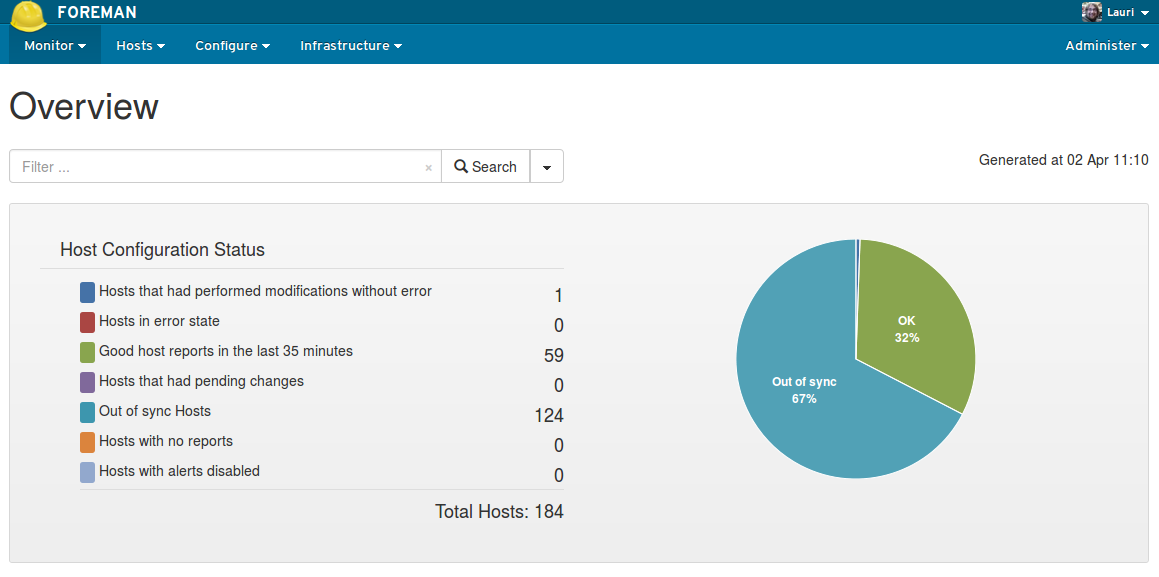
\includegraphics[scale=0.6]{img/foreman.png}}
\caption{Foreman}
\label{fig:digraph}
\end{figure}

Initially OpenLDAP was chosen for authentication and authorization,
but later we switched to Samba4 in order to provide better interoperability with
Windows workstations.
In fact Samba4 implements Microsoft Active Directory functionality to large extent,
making it possible to avoid licensing fees and 


\section{Transforming experience into service}

\subsection{Ubuntu deployment service}

As part of the major thesis a more efficient way of deploying Linux-based
workstations was devised.
The resulting software components were used to build an service for
distributing Linux-based operating system templates which can be used to
quickly deploy workstations, laptops and netbooks customized
for particular purpose.
Currently Koodur OÜ mainly maintains template of Ubuntu 14.04 LTS based
workstation which uses lightweight MATE desktop.

\begin{figure}[!htb]
\centering
\scalebox{0.5}{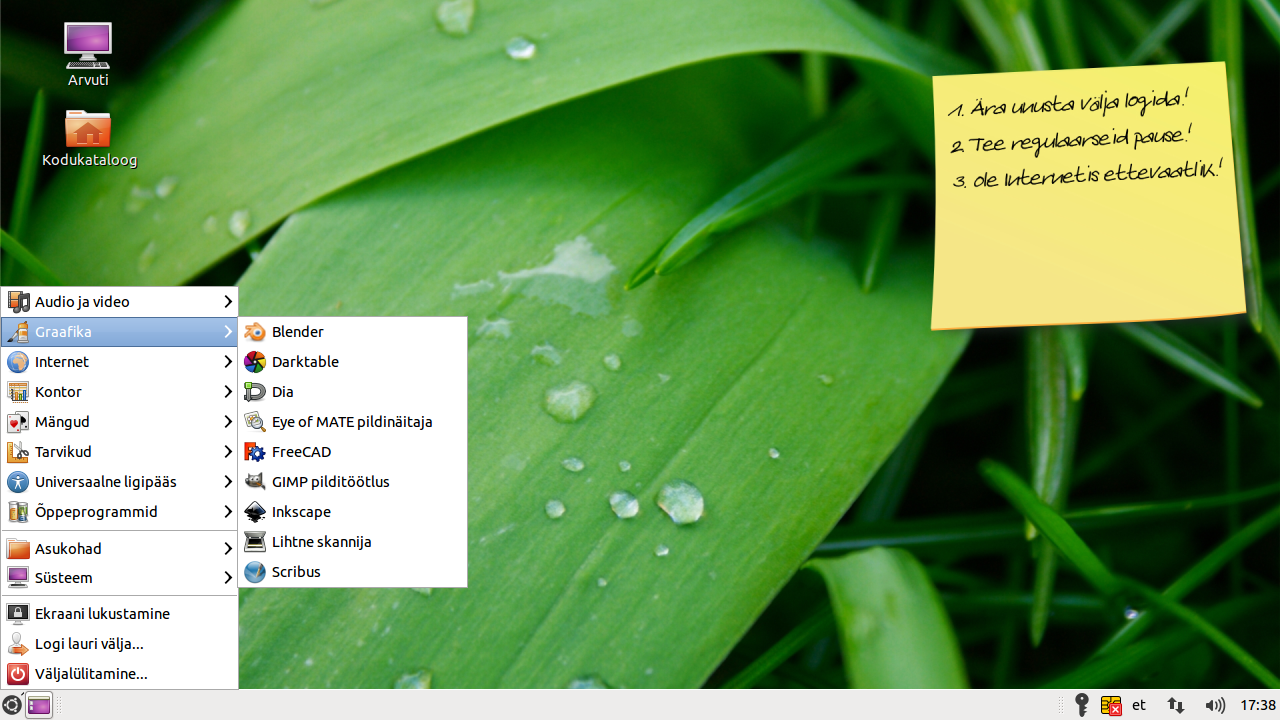
\includegraphics[scale=0.5]{img/edu-workstation}}
\caption{MATE desktop}
\label{fig:digraph}
\end{figure}

We've fine-tuned MATE to slightly mimic Windows XP layout to provide
familiar looks to older generation of users.


\subsection{Identity service}

Our customized Ubuntu 14.04 template integrates
well with existing Active Directory deployments
and Windows file shares.
We also provide Active Directory compatible
authenticationa and authorization service using Samba4.
This service is mainly targeted towards
smaller organizations lacking local
infrastructure and manpower to operate such services.

\subsection{ownCloud}

ownCloud is an open-source project which implements
Dropbox functionality to large extent.
In conjunction with out authentication service
we provide an ownCloud instance for our customers.



automatically associated with the Puppet master instance 
operated by us to apply security updates and configure the
deployed operating system.



  

As the Ubuntu is being continously improved it also requires
continous maintenance of the templates provided by the service.
Providing such service also requires extensive knowledge of
how the Linux-based operating system is put together of 
thousands of software components and how they interact with each other.


The educational institutions were used to bootstrap the service and gain
required experience to deliver enterprise grade service.



\section{Conclusion}


Snowden revelations pushed various governments to seek for alternatives
to relying on western technology.
For instance use of Windows 8 has been banned in German governmental agencies
\footnote{\url{http://blog.legalsolutions.thomsonreuters.com/law-and-techology/german-government-bans-windows-8-use-nsa-spying-puts-american-companies-risk/}}.

There is a vast pool of open-source tools available on the Internet to cater
various needs.
For instance Indian Govenrment mandates use of open-source technologies
in order to reduce total cost of ownership and to ensure
strategic control in e-Governance applications and systems in long run
\footnote{\url{http://deity.gov.in/sites/upload_files/dit/files/policy_on_adoption_of_oss.pdf}}.


\bibliographystyle{plain}
\bibliography{references}

\end{document}
